%
\DeclarePairedDelimiter\set\{\}
%=============================--A--=============================%
\subsection{1. Modulaç\~ao PSK}
\label{subsec:intro}
Na modulação por deslocamento de fase (\textit{phase-shift keying}) \textbf{os bits dos dados digitais são codificados numa forma analógica, ao modificar a fase da portadora sinusoidal}. Desta forma, múltiplos bits podem ser atríbuidos à onda portadora. 

A modulação PSK é definida pela seguinte equação:

\[ 
    s_m(t) = p(t)\cos{(2\pi f_c t + \theta_m)}\qquad m=1,\hdots,M
\]

Onde $\theta_m$ é o deslocamento de fase e $p(t)$ o \textit{pulse shaping signal}. O tipo mais comum de PSK é o \textit{binary phase-shift keying} (BPSK), em que um bit singular é atribuído à portadora. Em \textit{quadrature phase-shift keying} (QPSK), são mapeados dois bits em cada fase da portadora.

As modulações BPSK e QPSK são casos específicos da modulação PSK M-ária (M-PSK), com $M=2$ e $M=4$ respetivamente\footnotemark[1]. Os valores de fase da portadora são genericamente descritos no seguinte conjunto:

\footnotetext[1]{Onde $M \delequal$ número possível de fases da portadora $= 2^{\text{n\textsuperscript{\underline{o}}. bits}}$}

$$
    \set*{\frac{2\pi}{M}(m-1) + \varPhi}_{m=1}^{M}
$$
em que $\varPhi$ é uma constante de fase\footnotemark[2]. 

No âmbito laboratorial, são observadas as seguintes fases:

\footnotetext[2]{Atendendo aos mapeamentos no Guia de Laboratório, tem-se que $\varPhi \equiv 0$ para BPSK e $\varPhi \equiv \pi/4$ para QPSK.}

%\iffalse
$$
    \theta_m^{\text{BPSK}}= 
    \begin{cases}
        0\text{,}\ & \text{bit 1}\\
        \pi\text{,}\ & \text{bit 0}
    \end{cases}
    \quad \land \quad\
    \theta_m^{\text{QPSK}}= 
    \begin{cases}
        \pi/4\text{,}\ & \text{dibit 11}\\
        3 \pi/4\text{,}\ & \text{dibit 01}\\
        5 \pi/4\text{,}\ & \text{dibit 00}\\
        7 \pi/4\text{,}\ & \text{dibit 10}
    \end{cases}
$$
%\fi

\subsubsection{1.1 \textit{Constellation Modulator}}
\label{subsubsec:const-mod}
\begin{table}[h]
    \centering
    %\setlength{\extrarowheight}{1em}
    \begin{tabular}{c c}
        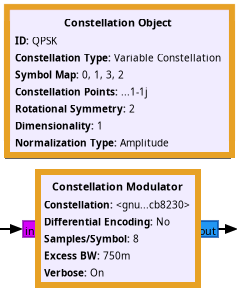
\includegraphics[scale=0.5,valign=c]{img/intro/constellation_mod.png} &\
        \raisebox{7\height}{\minipage[t]{0.65\linewidth-2\fboxsep-2\fboxrule\relax}
            No âmbito da modulaç\~ao em ambiente \textit{GNU Radio}:
            \\[0.2em]
            \hspace*{1em} "(...) The input is a byte stream (unsigned char) and the output is the complex modulated signal at baseband."\cite{constellationmodulator-gnuradio}
            \\[0.2em]
            \hspace*{1em} Pelo que o \textit{output} (que representa o sinal de banda-passante teórico em banda-base) proveniente do bloco \textit{Constellation Modulator} toma o seguinte formato\footnotemark[3]:
            $$ z(t) = I(t)+jQ(t) $$
        \endminipage}
    \end{tabular}
\end{table}

\footnotetext[3]{"Complex baseband equivalent representation of the real [passband] signal."\cite{mathuranathan_2020}}

\newpage
Pelo que

$$ 
    \sqrt{E_b} = \sqrt{\varepsilon} \delequal \sqrt{I(t)^2 + Q(t)^2} \;\; \land \;\; \theta(t) \delequal tan^{-1} \left( \frac{Q(t)}{I(t)} \right)
$$

Deste modo, a análise do sinal é passível de uma abordagem vetorial, como explicitado nos \hyperref[fig:constellations]{\textbf{diagramas de constelação} a baixo}:

\begin{figure}[H]
    \centering
    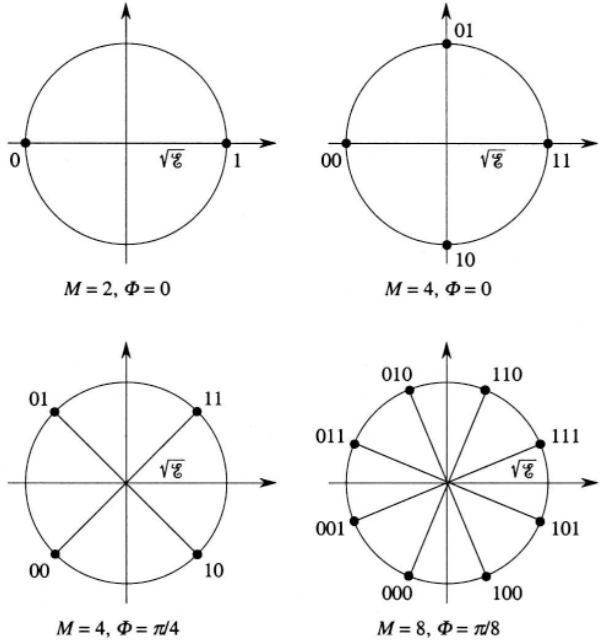
\includegraphics[width = 0.5\linewidth]{img/intro/gray-mapped_constellation.png}
    \caption{Representação geométrica de conjuntos de sinais PSK \textit{Gray-mapped}\cite{benedetto_biglieri_2002}.}
    \label{fig:constellations}
\end{figure}

O mapeamento dos símbolos para a representação em \textit{complex baseband} é garantido no bloco \textit{Constellation Object}. Atendendo ao parâmetro \textit{Variable Constellation}, para um ajuste fino, revela-se:
\begin{itemize}
    \item[] \underline{\textbf{Forma geral:}} \textit{Symbol Map} $\mapsto$ \textit{Constellation Points}
    \item[$\star$] \textbf{BPSK:} $[0, 1]\mapsto[-1, 1]$
    \item[$\star$] \textbf{QPSK:} $[0, 1, 3, 2]\mapsto[\underbrace{-1-1j}_{00},\underbrace{-1+1j}_{01},\underbrace{1+1j}_{11},\underbrace{1-1j}_{10}]$
\end{itemize}